\chapter{INTRODUCTION}
\label{ch:introduction}

\section{Background}
Recently the use of unmanned aerial systems (UAS) has increased dramatically in both civilian and military applications. Because of this, the Federal Aviation Administration (FAA) has been modifying the requirements for the operation of UAS. The one that concerns us is the line-of-sight (LOS) requirement, which constrains the aircraft mission to be within the visual field of the operator. The existing method is to keep an eye on the aircraft with binoculars, which is prone to lose the plane frequently. The importance of UAS tracking systems relies on having a good link between the aircraft and the ground control station (GCS), which can be assured using a good antenna pointing system.

Another critical requirement in the reliability of a UAS mission is the communication with the ground station. For reliable communication it is necessary to point the antenna towards the UAS and maintain the LOS with the aircraft. Therefore, the communication link will be strong as long as we have LOS. This is apparent for applications that require real-time feedback, because if the tracking of the UAS is not accurate, the link could be interrupted and no feedback would be sent back. An example is a military mission where an aircraft supports an advancing troop in enemy territory.  The decisions made by the leader of the troop are greatly influenced by the feedback of the UAS. If the communication between the UAS and the GCS is lost, there would not be any feedback from the UAS and the safety of the soldiers could be compromised. Moreover, in a civilian application such as disaster relief for an earthquake, the aircraft could be equipped with a thermal imaging camera to detect heat sources. It would identify warm bodies under the rubble in real time so the help could get there as soon as possible. If the communication is lost between the UAS and the GCS, some information might be missed that could lead to the detection of a survivor.

\section{Contributions}
\begin{figure}[h!]
  \centering
  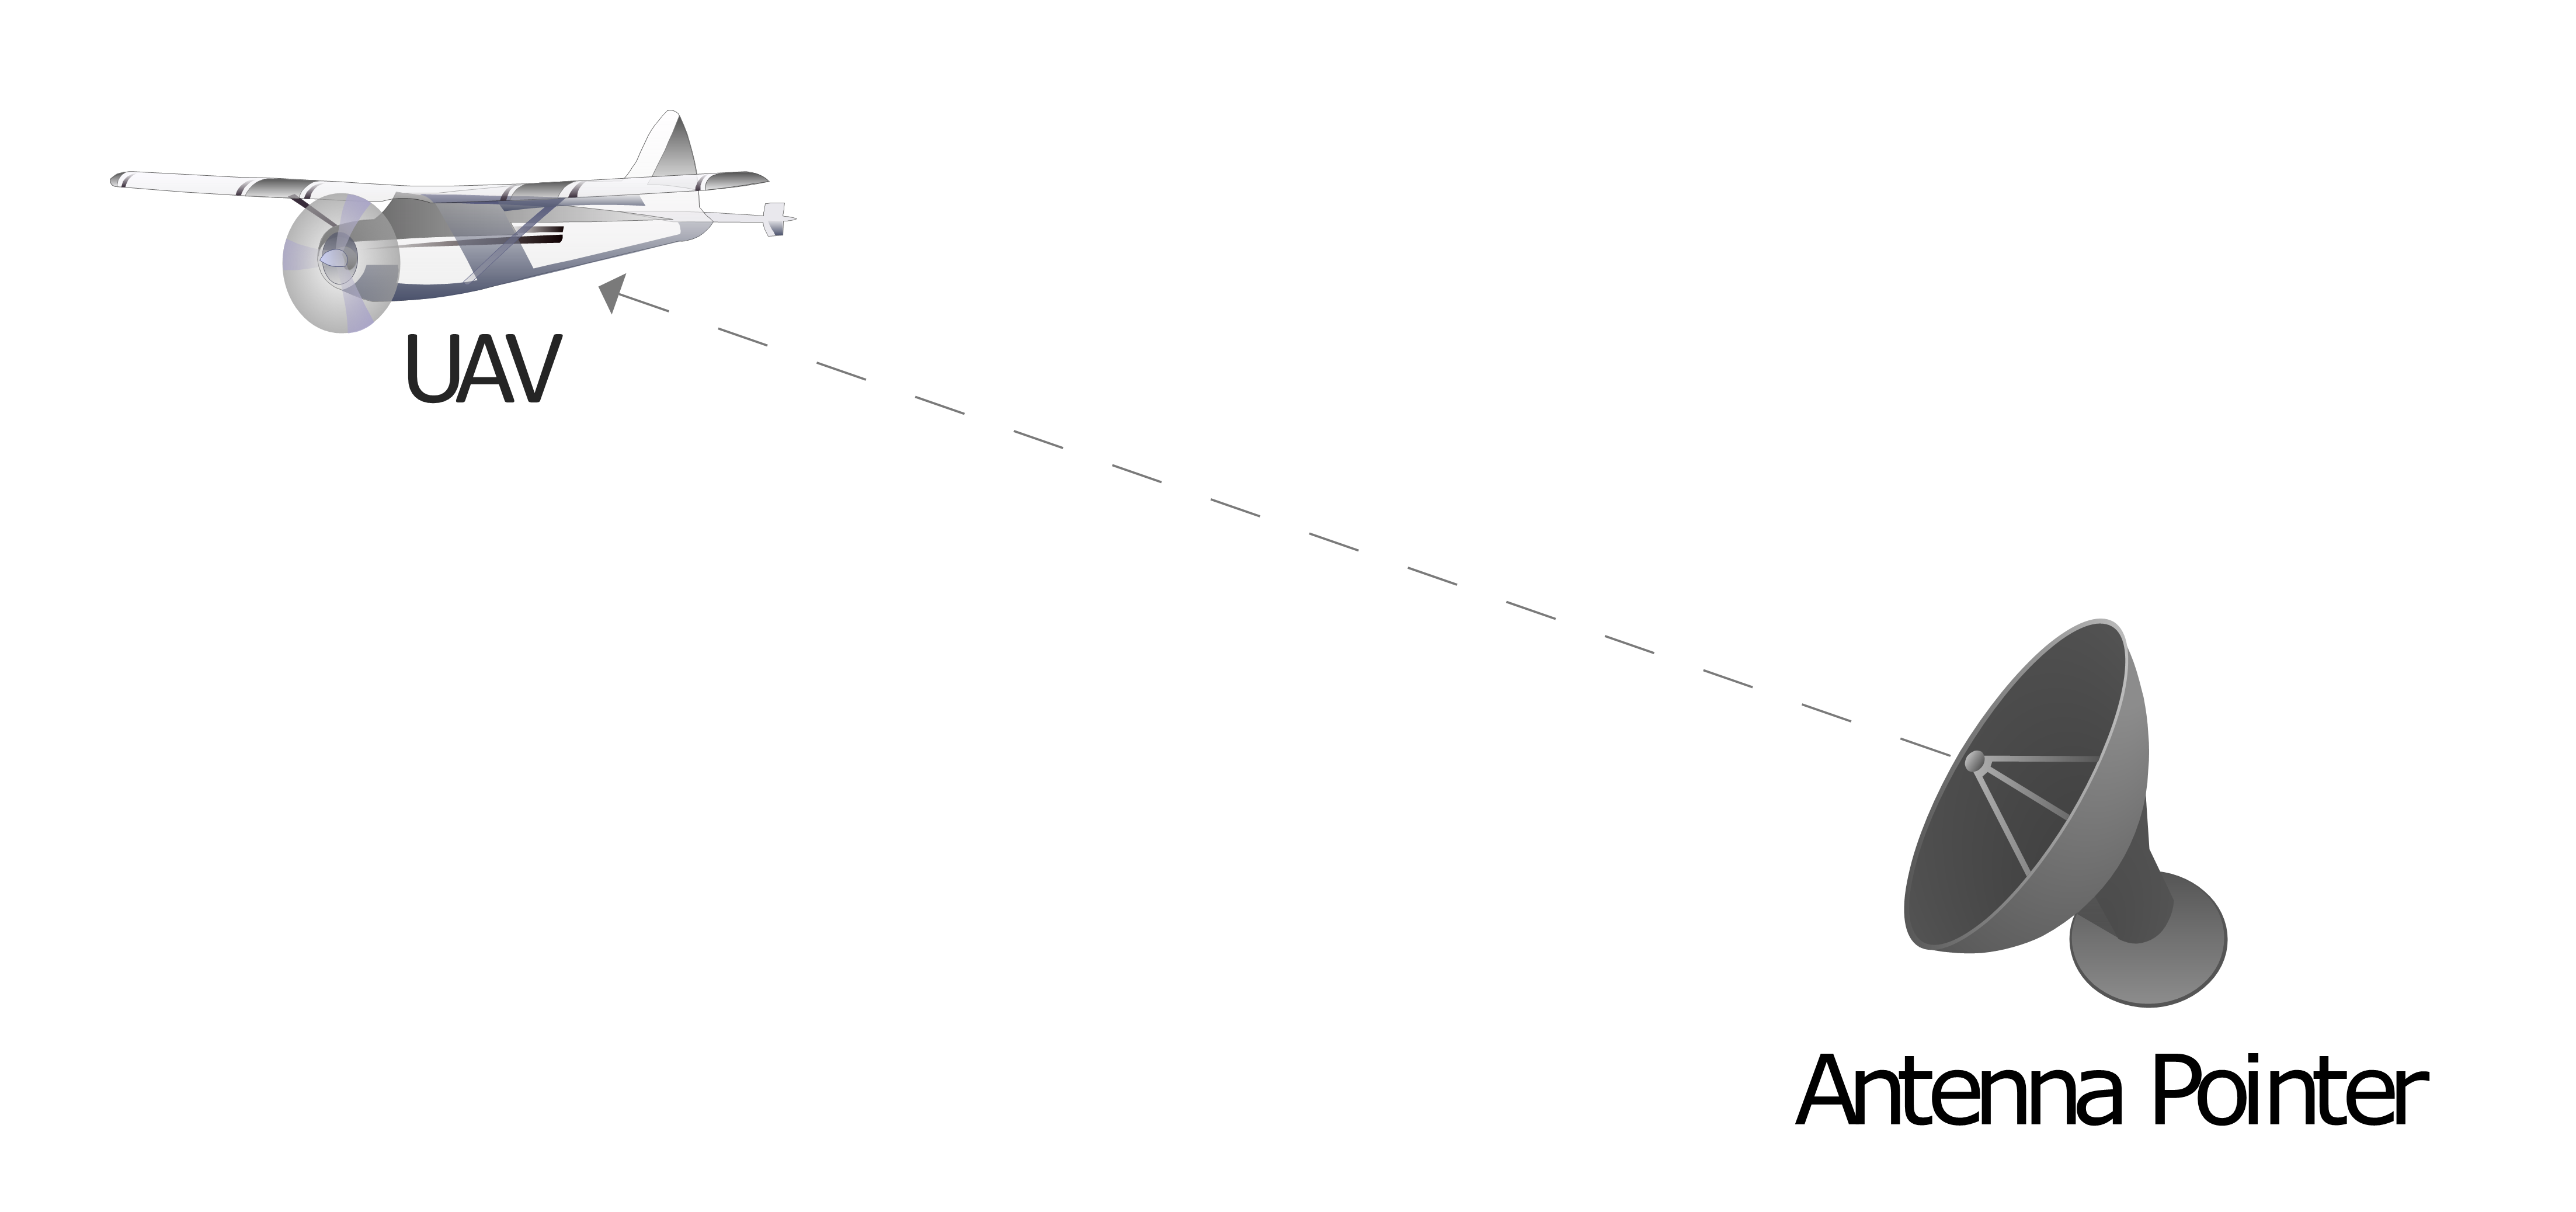
\includegraphics[scale=.075]{./Diagrams/AP_UAV}
  \caption{Antenna Pointer tracking an UAS}
\end{figure}
The main focus of this work is to design an autonomous system to point an antenna mounted with a camera towards a flying UAS to maintain communication and visual LOS to satisfy FAA requirements. In order to point a camera, the precise position of the aircraft is required. The existing approach is for the GCS to use the position obtained from a GPS receiver on board the UAS. There are several limitations of this approach. 
\begin{itemize}[nosep]
\item The GPS receives position updates at 1-4 Hz, not fast enough to point the antenna towards an UAS flying at 20 m/s.
\item The position updates at the antenna are delayed and have out-of-sequence measurements (OOSM) due to communication delays.
\end{itemize}
\begin{figure}[h!]
  \centering
  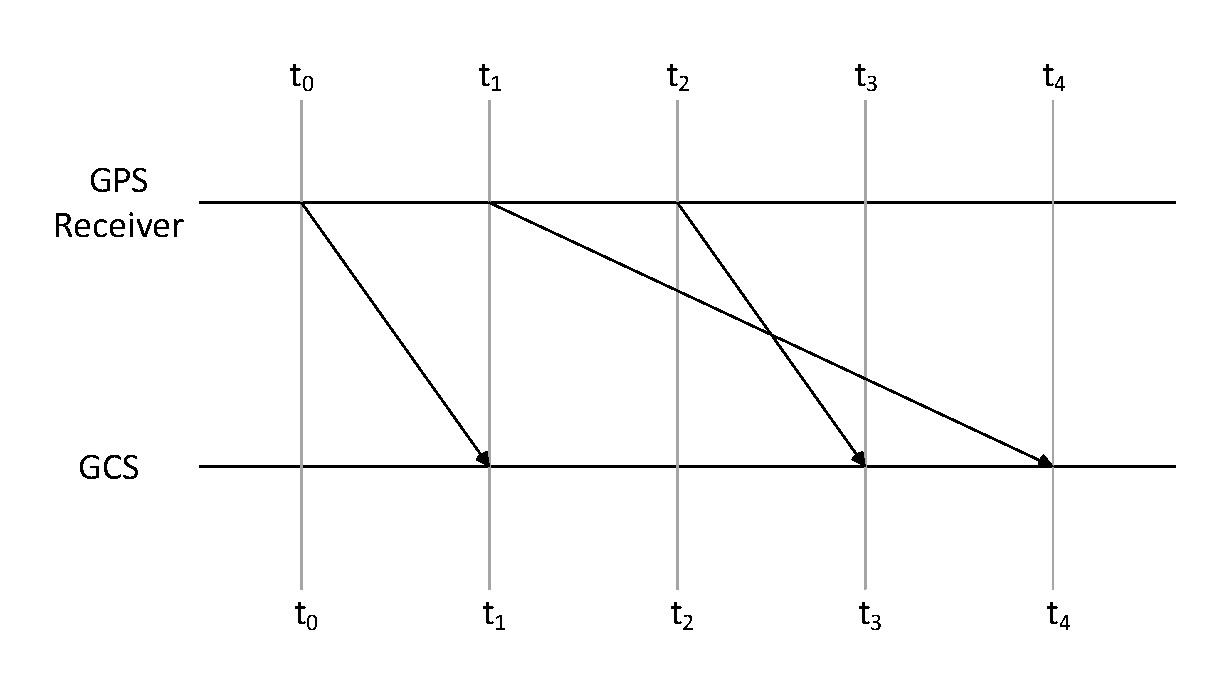
\includegraphics[scale=.37]{./Diagrams/OOSM}
  \caption[Out-Of-Sequence Measurement]{OOSM. 
  In this diagram the generation time of various measurements (GPS receiver line) and the time that they are available to the system (GCS line) are shown. Measurements $t_1$ and $t_2$ are out-of-sequence since $t_2$ is available first than $t_1$.\label{fig:OOSM}}
\end{figure}
A measurement is called out-of-sequence if it is available to a processing unit first than another measurement taken in an earlier time step. This situation is shown in figure \ref{fig:OOSM}.

The first problem is addressed by adding a camera which provides location measurements from images of the aircraft at 30 Hz, compensating the slow update rate of GPS. However, the camera's accuracy deteriorates with distance, since at higher distances the aircraft would only be a couple of pixels in the camera image, making the recognition of the UAS impossible. On the other hand, GPS measurements' errors are independent of the distance between the fixed wing and the antenna pointer, making the relative error smaller at higher distances. Hence, we can say that the camera and GPS are complementary sensors for pointing the antenna. The second problem of receiving out of sequence measurements is addressed by using an extended Kalman filter which uses out of sequence GPS measurements with camera measurements to estimate the position of the UAS. This estimation is then used to reliably point the antenna and camera towards the aircraft.

\pagebreak
\section{Literature Review}
For more than two decades, the problem of OOSM have been addressed in several different ways. The initial studies about the OOSM are presented in \cite{Hilton1993} in 1993, where a negative-time update technique is developed using the criterion of minimum mean-square error. The first optimal algorithm for the general multi-step lag problem appeared in \cite{Nettleton2001} in 2001. It consisted in buffering all the measurements received and running the filter behind real-time. Consequently, this algorithm is not able to run in real time. In \cite{Larsen1998}, a solution of this problem is presented, in which a new filter is developed where the measurements are extrapolated forward in time using past and present estimates to calculate an optimal gain for the Kalman filter. The work of \cite{Larsen1998} is expanded in \cite{Julier2005}, where a covariance union method is proposed to solve the multi-lag OOSM when the delay is not precisely known. In \cite{Mallick2001} a linear minimum variance estimation algorithm was extended to handle multiple lags and dynamics models. This exposed that as the number of lags increases, the state estimation accuracy decreases. The same problem is addressed in \cite{Bar-Shalom2002a}. The one-step lag OOSM solution is generalized to solve problems when multiple lags arise. This extension comes with a significantly lower storage requirement and a small (1\%) degradation of MSE performance. A two-step method was presented in \cite{Lanzkron2004} which requires one more step to update the state at the OOSM time. Two optimal algorithms were presented in \cite{Zhang2002} to approach the multi-step OOSM problem using fixed-point smoothing. It was shown that both of these algorithms are flexible and relatively simple but highly computationally demanding. In \cite{Bar-Shalom2002} the exact state update equation for the OOSM problem is presented and compared to two suboptimal algorithms. Each method is tied to the situations where they should be used comparing simplicity against optimality. A smoothing-based algorithm was proposed in \cite{Mallick2002} in the case of multi-sensor multi-target ground moving target tracking problem. It concluded that discarding OOSM can lead to severe degradation in the state estimation. Also these two methods have better accuracy than the previous buffering method approach. A unified sub-optimal Bayesian approach is proposed in \cite{Challa2002} for the multi-lag OOSM problem. This algorithm, developed on the basis of a fixed-lag smoothing framework and its solution reduces to an augmented state Kalman filter. An extension of the particle filter approach can be found in \cite{Orton2005} where it compares it results with the extended Kalman filter, showing that both have similar performance. The work of \cite{Plett2007} develops an out-of-order sigma-point Kalman filter for solving the multi-lag OOSM in a single measurement vector and using the batch-form update. This method is equivalently complex per iteration as the sigma-point Kalman filter but it requires more iterations. An extended Kalman filter was used to estimate the position of a UAS using a camera and then coupled with an inertial measurement unit (IMU). The results shown that coupling the camera with an IMU reduces the position estimation error by almost and order of magnitude, compared to using only the camera \cite{Kelly2008}. In \cite{Zhang2012} three different approaches were proposed to achieve optimality. The study yielded that the complete in-sequence information fixed point smoothing method was the optimal approach, but it lacks simplicity. 

The work of this thesis is developed by combining the delayed Kalman filter of \cite{Larsen1998} and the extended Kalman filter explained in \cite{Beard2010a}. Both techniques are combined in a filter with a nonlinear model of the system that can handle delays. Moreover, random delays and the OOSM problem will be handled by the modified filter. The estimation errors will be compared for different GPS measurement delays, fixed and randomized, as well as using GPS alone or coupled with a camera. Also, for comparison purposes, the estimation is done by an extended Kalman filter which will not take into account the delays or the OOSM problem. Therefore, the major contribution of this study is to clearly show the increase in accuracy that comes from using this delayed extended Kalman filter.